\documentclass[10pt, a4paper]{article}

\usepackage{hyperref}
\usepackage{listings}
\usepackage{todonotes}
\usepackage{graphicx}
\usepackage[section, below]{placeins}

\parindent 0pt

\title{Documentation of Nirs Analysis Scripts}
\author{L.Beichert@stud.uni-heidelberg.de}
\date{\today}


\begin{document}
\maketitle

\section{Requirements}
The scripts work with nirs/systemic(/phosphorus) data structs as they are created by the nirs data synchronisation scripts (\url{https://github.com/aot/ucl-nirs-analysis}).
The data structs are expected to be save into files called 'pigData.m'.
\todo{tools in path}

\section{overviewPlots}
Used like:

\begin{lstlisting}
>> overviewPlots(pigDataNTB)
\end{lstlisting}

Creates an overview plot of every subject in the data-struct 'pigDataNTB' (use loadData to load) and saves it as .pdf and .fig file under \url{overviewPlots/output/}.

\begin{figure}[h]
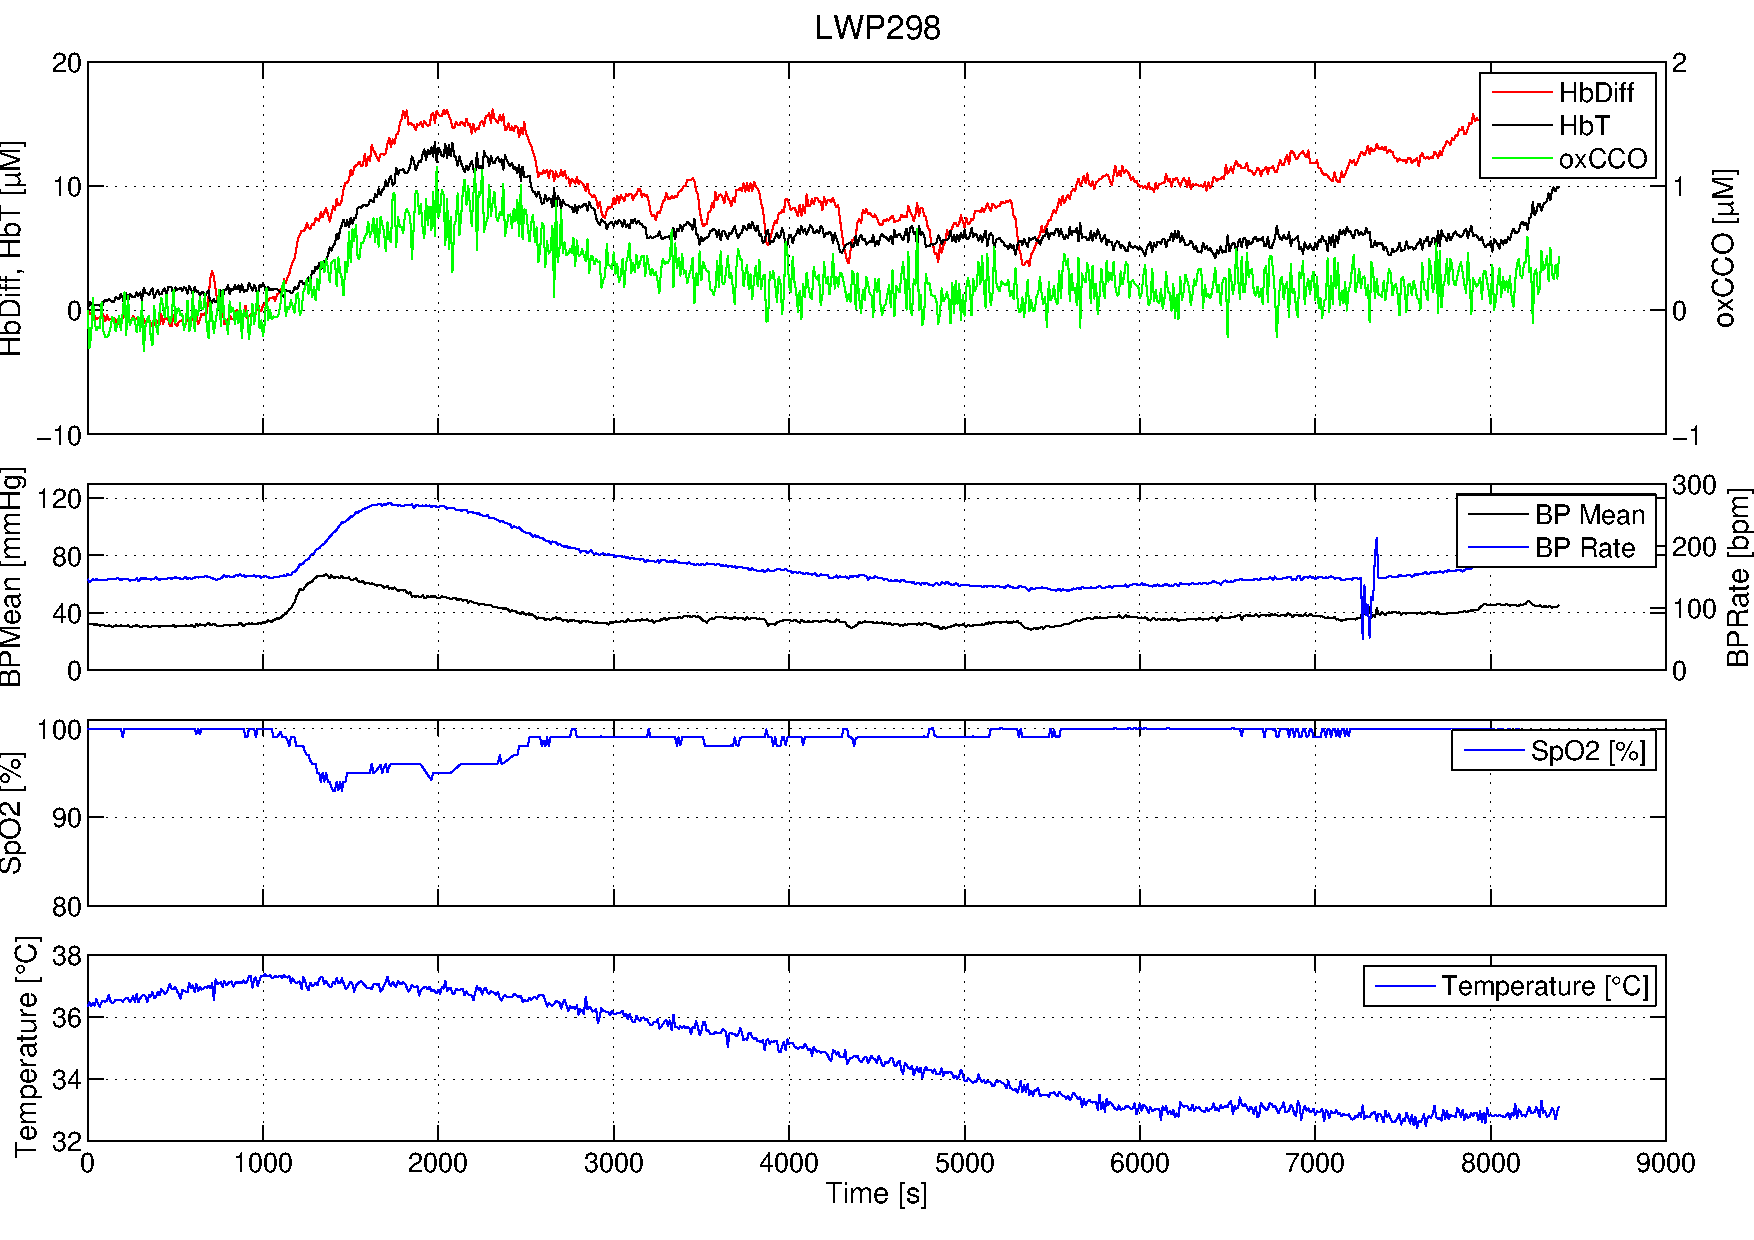
\includegraphics[width=0.9\textwidth]{LWP298_Argon_Raw.pdf}
\caption{Sample overview plot created with overviewPlots}
\end{figure}


\section{diffsBeforeAfter}

\section{recoveryFraction}

\section{tools}
\subsection{loadData(suffix)}
Used like:

\begin{lstlisting}
>> loadData('31p')
\end{lstlisting}

Loads pigData-structs of type 'suffix'(31p, 1h, cooling, ...) into workspace variable 'pigDataNTB'. 

Expects the structs to be saved as files called 'pigData.m' under the location \url{pigletdatadir/argon-dex/output/suffix/}. The path to the data directory must be saved as MATLAB-appdata 'pigletdatadir'. This can be done by copying the 'startup.m' file from \url{/tools} to the home directory of MATLAB and editing it according to the local path or by integrating the lines into a pre-existing startup-file. 



\end{document}
